\documentclass[12pt, oneside]{article}
\usepackage[letterpaper, margin=1in, headsep=0.5in]{geometry}
\usepackage[english]{babel}
\usepackage[utf8]{inputenc}
\usepackage{amsmath}
\usepackage{amsfonts}
\usepackage{amssymb}
\usepackage{tikz}
\usetikzlibrary{quotes, angles}
\usepackage{graphicx}
%\usepackage{pgfplots}
%\pgfplotsset{width=10cm,compat=1.9}
%\usepgfplotslibrary{statistics}
%\usepackage{pgfplotstable}
%\usepackage{tkz-fct}
%\usepackage{venndiagram}

\usepackage{fancyhdr}
\pagestyle{fancy}
\fancyhf{}
\rhead{\thepage \\Name: \hspace{1.5in}.\\}
\lhead{BECA / Dr. Huson / 10th Grade Geometry\\* 15 November 2018}

\renewcommand{\headrulewidth}{0pt}

\begin{document}
\subsubsection*{Classwork assessment: Isosceles base theorem}
Show each step, justify each by writing the name of a theorem to the right.  
\begin{enumerate}

  \item Given $\triangle ABC$. $\overline{AC} \cong \overline{BC}$,  $m\angle A=55$. Find $m\angle C$.\\[0.5cm]
    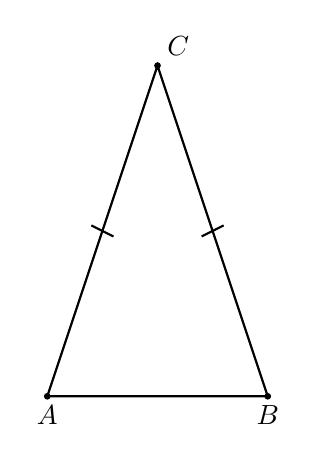
\begin{tikzpicture}[scale=0.7]
      \draw [thick](0,0)--(4,0)--(2,6)--(0,0);
      \draw [fill] (0,0) circle [radius=0.05] node[below]{$A$};
      \draw [fill] (4,0) circle [radius=0.05] node[below]{$B$};
      \draw [fill] (2,6) circle [radius=0.05] node[above right]{$C$};
      %\draw [color=blue] (0,0) ++(0.75,0) arc [start angle=0, end angle=70, radius=0.75];
      %\draw [color=blue] (4,0) ++(-0.22, 0.73) arc [start angle=110, end angle=180, radius=0.75];
      \draw [thick] (0.8,3.1)--(1.2,2.9); %tick mark
      \draw [thick] (2.8,2.9)--(3.2,3.1); %tick mark
      %\node [right] at (3.25,2.5){$x+7$};
      %\node [left] at (0.75,2.5){$2x+1$};
    \end{tikzpicture}%\vspace{1cm}

  \item Given $\triangle DEF$. $\overline{DF} \cong \overline{EF}$,  $m\angle F=72$. Find $m\angle D$.\\[0.5cm]
    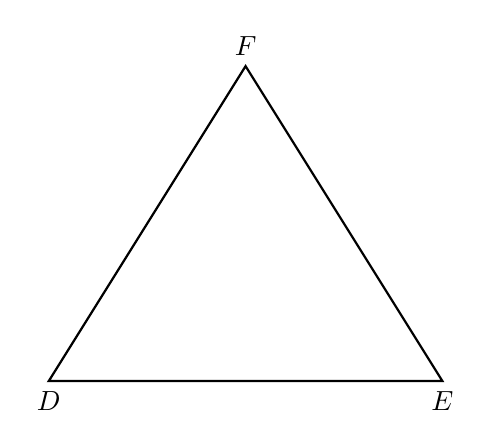
\begin{tikzpicture} %[scale=3] Isosceles, parallel marks, congruence marks
      \draw [-, thick] (0,0) node[below]{$D$}--
        (5,0) node[below]{$E$}--(2.5,4) node[above]{$F$}--cycle;
      %\draw [>->, thick] (1.0,1.6)--(1.25,2);
      %\draw [{Bar[]}-{Bar[]}, thick] (4,1.6)--(3.75,2);
      %\draw [color=blue] (0.75,0) arc [start angle=0, end angle=58, radius=0.75];
      %\draw (5,0)-- +(-0.75,0) arc [start angle=180, end angle=122, radius=0.75];
    \end{tikzpicture}%\vspace{1cm}

  \item Given the triangle shown with congruent sides marked.  $m\angle 1=110$. Find $m\angle 2$\\
  Spicy: Find the measure of the vertex angle. \\[0.5cm]
    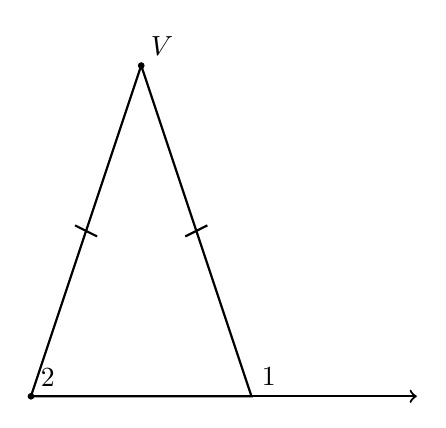
\begin{tikzpicture}[scale=0.7]
      \draw [thick](0,0)--(4,0)--(2,6)--(0,0);
      \draw [->, thick](0,0)--(4,0) node[above right]{1}--(7,0);
      \draw [fill] (0,0) circle [radius=0.05] node[above right]{$2$};
      %\draw [fill] (4,0) circle [radius=0.05] node[below]{$B$};
      \draw [fill] (2,6) circle [radius=0.05] node[above right]{$V$};
      %\draw [color=blue] (0,0) ++(0.75,0) arc [start angle=0, end angle=70, radius=0.75];
      %\draw [color=blue] (4,0) ++(-0.22, 0.73) arc [start angle=110, end angle=180, radius=0.75];
      \draw [thick] (0.8,3.1)--(1.2,2.9); %tick mark
      \draw [thick] (2.8,2.9)--(3.2,3.1); %tick mark
      %\node [right] at (3.25,2.5){$x+7$};
      %\node [left] at (0.75,2.5){$2x+1$};
    \end{tikzpicture}

\newpage
    \item Given circle $Z$ with inscribed $\triangle XYZ$. $m\angle Z=100$. Find $m\angle Y$.\\[1cm]
        %\hspace{1cm} Given the line  $l$ and point $P$.
        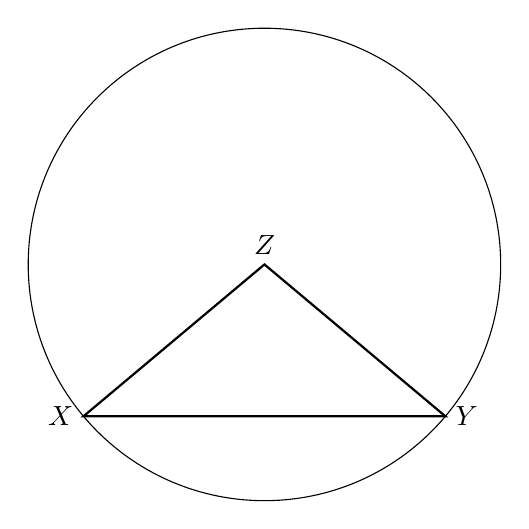
\begin{tikzpicture}
          %\draw [-, thick] (-6,0) node[left]{$A$}--(0,0);
          \draw  (0,0) circle [radius=3] node[above]{$Z$};
          \draw [-, thick] (220:3) node[left]{$X$}--(0,0)
            --(320:3) node[right]{$Y$}--cycle;
          %\node at (8.5,-0.4){$l$};
          %\draw [fill] (6,0) circle [radius=0.05] node[below]{$Q$};
        \end{tikzpicture}

    \item Given circle $O$ with inscribed $\triangle SLO$. $m\angle S=x+7$. Find $m\angle O=2x-2$. Find $x$.\\
    For full credit, check your answer.\\[1cm]
        %\hspace{1cm} Given the line  $l$ and point $P$.
        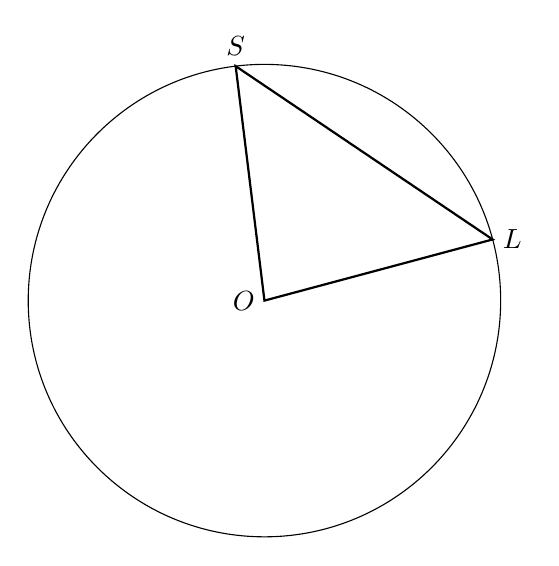
\begin{tikzpicture}
          %\draw [-, thick] (-6,0) node[left]{$A$}--(0,0);
          \draw  (0,0) circle [radius=3] node[left]{$O$};
          \draw [-, thick] (15:3) node[right]{$L$}--(0,0)
            --(97:3) node[above]{$S$}--cycle;
          %\node at (8.5,-0.4){$l$};
          %\draw [fill] (6,0) circle [radius=0.05] node[below]{$Q$};
        \end{tikzpicture}
        \vspace{1cm}
    \item Writing to learn: Why do we write down the theorems that justify each step to solve a problem?

\end{enumerate}
\end{document}
